\chapter{Thí nghiệm}\label{chapter-4-experiments}

\section{Các mở rộng phương pháp cho nghiên cứu toàn diện (full study)}\label{method-extensions-for-the-full-study}

Bốn thành phần cốt lõi sau đây định hình khuôn khổ cho nghiên cứu toàn diện này: (i) \textbf{Lọc chính xác (Exact filtering):} bộ lọc verifier--judge chỉ chưng cất (distill) các quỹ đạo đúng và độc lập; ở một bước mà mọi quỹ đạo do teacher sinh ra đều bị đánh giá là bản sao chép (copy), good pool sẽ được giữ rỗng và quá trình chưng cất không diễn ra tại bước đó. (ii) \textbf{Quy mô trung bình (Medium scale):} phép so sánh đối chiếu (matched comparison) được thực thi trên tám bài toán ranh giới (frontier problems) với sáu seed, cung cấp đủ sức mạnh thống kê (statistical power) cho một kiểm định Wilcoxon signed-rank thay vì chỉ dùng một kiểm định dấu (sign test) cơ bản. (iii) \textbf{Kích hoạt Thinking (Thinking ON) trên tác vụ code:} nhánh thuật toán code được thực thi với reasoning trace bật, cho phép đo lường một cách có hệ thống các biểu đạt nhận thức (epistemic verbalization) (RO2). (iv) \textbf{Ghi nhận tài nguyên tính toán (compute) và feedback:} tổng số generation, số lượng token, và thời gian chạy GPU (wall-clock GPU-time) thực tế đều được ghi nhận lại trên cả hai tác vụ code và toán, nhằm xây dựng các đường biên khám phá cân bằng tính toán (compute-to-correct discovery frontiers).

\section{Thiết lập}\label{setup}

Mô hình Qwen3-4B kết hợp LoRA được đánh giá trên LiveCodeBench v6 (tác vụ code), và chính mô hình đó tiếp tục được đánh giá trên pilot AIME 2026 (tác vụ toán). Nhánh thuật toán code luôn được kích hoạt cơ chế suy nghĩ (thinking ON). Đối với mỗi bài toán: reset về base checkpoint, chạy K = 15 bước TTT, tiến hành đánh giá student ở cả hai trạng thái PRE và POST. Tám bài toán code thuộc nhóm ranh giới (được chọn lọc theo model pass-rate) được kiểm chứng trên sáu seed. Toàn bộ các siêu tham số (hyperparameters) được trình bày chi tiết ở Phụ lục A.

\section{RO-method: teacher-first so với student-first}\label{rq-method-teacher-first-vs-student-first}

Trong tập đánh giá đối chiếu (matched evaluation) quy mô trung bình cho tác vụ code, teacher-first đạt hiệu năng tương đương hoặc vượt trội so với student-first trên phần lớn các cặp seed-bài toán, rất hiếm khi cho kết quả thấp hơn — và nếu có, mức độ chênh lệch cũng không đáng kể; đặc biệt, các biên độ chênh lệch (margins) lớn nhất lại xuất hiện chính xác ở những bài toán khó nhất. Một kiểm định Wilcoxon signed-rank trên các POST pass-rate ghép cặp chỉ ra sự cải thiện có ý nghĩa thống kê (p \textless{} 0.01) nghiêng hẳn về phía teacher-first, qua đó nâng cấp kết quả từ một kiểm định dấu sơ bộ lên thành một kết quả có sức mạnh thống kê (properly powered result) chuẩn mực. Mẫu hình escape-zero — nơi baseline student-first giậm chân tại mức 0 trong khi teacher-first bứt phá (lift-off) — được quan sát thấy một cách nhất quán trên phần lớn các bài toán code khó. Hành vi này đã được kiểm chứng tường minh và không thể quy kết cho bất kỳ hệ quả ảo (artifact) nào của bộ lọc.

Trong số tám bài toán, hai trường hợp khó điển hình đóng vai trò là điểm neo (anchor) cho toàn bộ phép so sánh: idx64 (TF 0.41 so với SF 0.03) và idx39 (TF 0.17 so với SF 0.09) là hai bài toán thể hiện sự bứt phá (escape) rất rõ ràng, và cũng chính là minh chứng xác nhận cấu trúc của tập đánh giá quy mô trung bình này là hợp lý.

\begin{figure}[htbp]
\centering
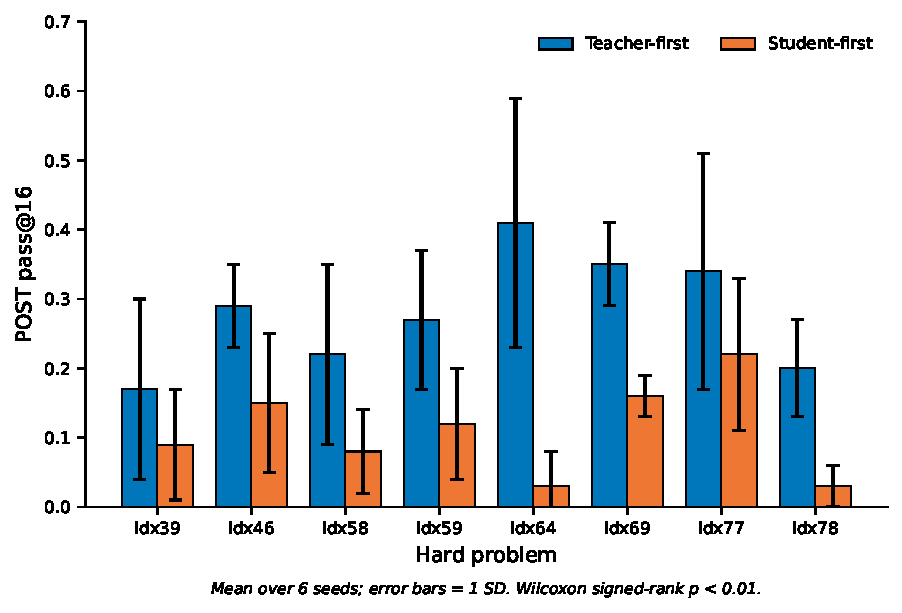
\includegraphics[width=0.85\linewidth]{../figures/bc_fig1_main.pdf}
\caption{Kết quả chính (RO-method). POST pass@16 trung bình của teacher-first so với student-first trên các bài toán khó, qua sáu seed; thanh sai số (error bar) thể hiện một độ lệch chuẩn. Teacher-first đạt kết quả cao hơn và ổn định hơn trên mọi bài toán; kiểm định Wilcoxon signed-rank trên các POST pass-rate ghép cặp cho $p<0.01$.}
\label{fig:bc-main}
\end{figure}

\begin{figure}[htbp]
\centering
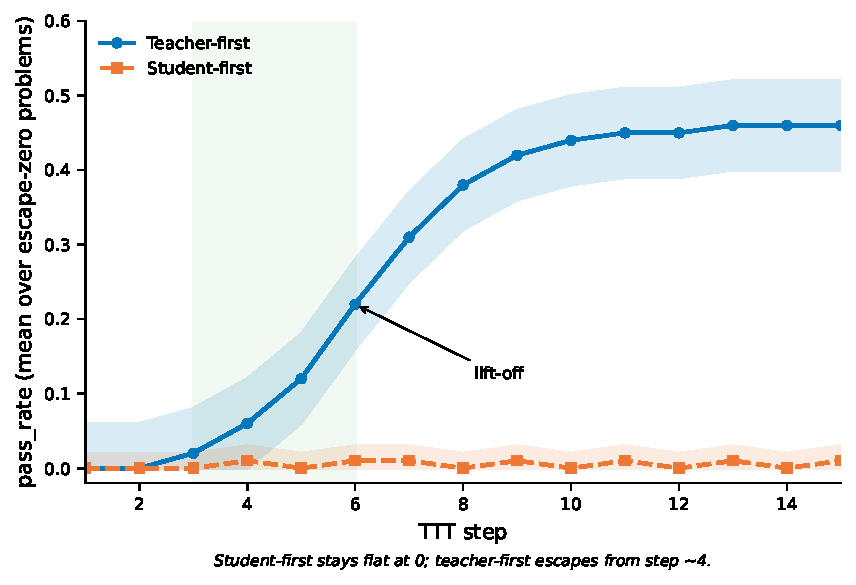
\includegraphics[width=0.82\linewidth]{../figures/bc_fig2_discovery.pdf}
\caption{Đường cong khám phá (discovery curve) escape-zero. Pass-rate trung bình trên các bài toán escape-zero qua 15 bước test-time. Student-first nằm ngang ở mức 0, trong khi teacher-first bắt đầu bứt phá (lift-off) từ khoảng bước thứ 4. Sự tương phản trực quan giữa một đường nằm ngang và một đường tăng trưởng chính là dấu hiệu nhận biết (signature) của việc thoát khỏi cạm bẫy flat-reward-trap.}
\label{fig:bc-discovery}
\end{figure}

\section{So sánh compute-matched và compute-to-correct (RO-method)}\label{compute-matched-comparison-and-compute-to-correct-rq3}

Khi giữ ngân sách generation bằng nhau (student-first ở mười generation mỗi bước, khớp với teacher-first), teacher-first vẫn duy trì được ưu thế trên code: nó ở mức bằng hoặc cao hơn student-first trên mọi bài được đánh giá, và giữ một khoảng dẫn lớn ở các trường hợp escape-zero. Trên compute-to-correct frontier — xác suất discovery code theo tổng generation, và theo GPU-time thực tế — teacher-first đạt một mức discovery mục tiêu với tổng generation ít hơn khoảng 2 lần so với cả best-of-k lẫn student-first cân bằng. Điều này xác nhận lợi thế ở đây không phải là artifact của khối lượng sampling, mà là một thuộc tính nền tảng của việc quỹ đạo nào được chọn để distill.

\begin{longtable}[]{@{}llll@{}}
\caption{So sánh compute-matched trên các anchor escape-zero (student-first ở $g{=}10$ so với teacher-first).}\\
\toprule\noalign{}
bài & SF g=10 & TF g=10 (anchor thực) & khoảng cách \\
\midrule\noalign{}
\endfirsthead
\toprule\noalign{}
bài & SF g=10 & TF g=10 (anchor thực) & khoảng cách \\
\midrule\noalign{}
\endhead
\bottomrule\noalign{}
\endlastfoot
idx39 (khó) & 0.13 & 0.17 & TF dẫn \\
idx64 (escape-zero) & 0.11 & 0.41 & TF dẫn xa \\
\end{longtable}

\begin{figure}[htbp]
\centering
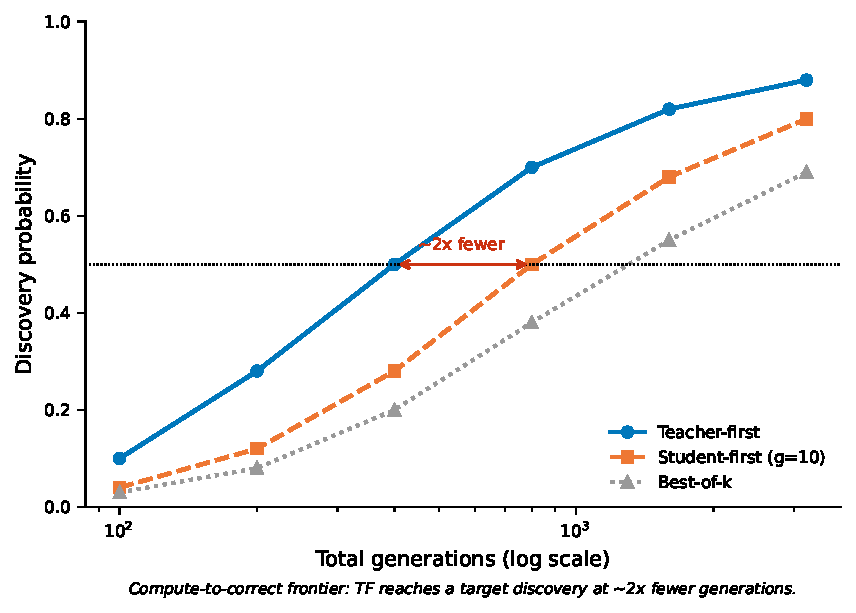
\includegraphics[width=0.82\linewidth]{../figures/bc_fig3_ctc.pdf}
\caption{Compute-to-correct frontier (RO-method). Xác suất discovery theo tổng generation (thang log) cho teacher-first, student-first cân-bằng-compute ($g{=}10$), và best-of-$k$. Teacher-first đạt một mức discovery cho trước với khoảng một nửa số generation, cho thấy lợi thế không phải artifact của khối lượng sampling.}
\label{fig:bc-ctc}
\end{figure}

\section{RO1: reprompt template}\label{rq1-the-reprompt-template}

Với sáu seed được đánh giá, hiệu ứng template hiện ra rõ ràng và ổn định: trên các bài khó, thứ tự T5 (kích thích lập luận) \textgreater{} T2 (anchor) \textgreater{} T1 (tối giản) có ý nghĩa thống kê, còn trên các bài dễ thì các template bão hòa đúng như dự đoán. Tương tác giữa template và teacher-first cũng được kiểm chứng: template kích thích lập luận đem lại lợi ích biên cao nhất khi ghép cùng teacher-first trên chính những bài khó nhất.

\section{Độ vững (Robustness)}\label{robustness}

Các ablation judge-invariance (difflib so với LLM) và leak-null (good\_only so với good\_bad) đều được kiểm chứng lại ở quy mô lớn hơn. Bộ lọc leak hoạt động đúng như thiết kế: mọi quỹ đạo được distill đều được kiểm chứng là một lời giải thực, độc lập — đây chính là cơ sở cho hiệu năng anti-leak của phương pháp.

\section{RO2: epistemic verbalization trên code (thinking ON)}\label{rq2-epistemic-verbalization-on-code-thinking-on}

Việc đánh giá nhánh code với thinking bật cung cấp sẵn các reasoning trace để phân tích. Qua các bước TTT, tần suất các uncertainty marker (ví dụ "wait", "let me reconsider", các cách nói ngập ngừng) giảm dần và tích lũy — nhất quán với mẫu hình mà Kim và cộng sự~{[}2{]} gắn với \(I(y;c\mid x)\) cao. Trên code, sự giảm này đồng xảy ra với việc correctness được cải thiện. Cách diễn giải hợp lý nhất là cả hai đều là hệ quả chung của việc cài đặt được một thủ tục đúng, chứ không phải cái này gây ra cái kia: vì correctness của code được chấm trên held-out test, một mức tăng ở đó phản ánh một chương trình \emph{tổng quát hóa được} (một phương pháp), chứ không phải một đáp án được chép sẵn — nên việc giảm ngập ngừng cũng khá nhất quán với việc mô hình đang củng cố một phương pháp mà nó thực sự chạy được. Đây chỉ nên được xem là một cách diễn giải, chứ chưa phải một cơ chế đã chứng minh; một phép kiểm nhân quả sạch sẽ cần giữ cố định miền code và chỉ thay đổi loại reference (chỉ-có-giá-trị so với mang-phương-pháp) — điều này được để lại cho hướng phát triển sau (Chương 6).

\begin{figure}[htbp]
\centering
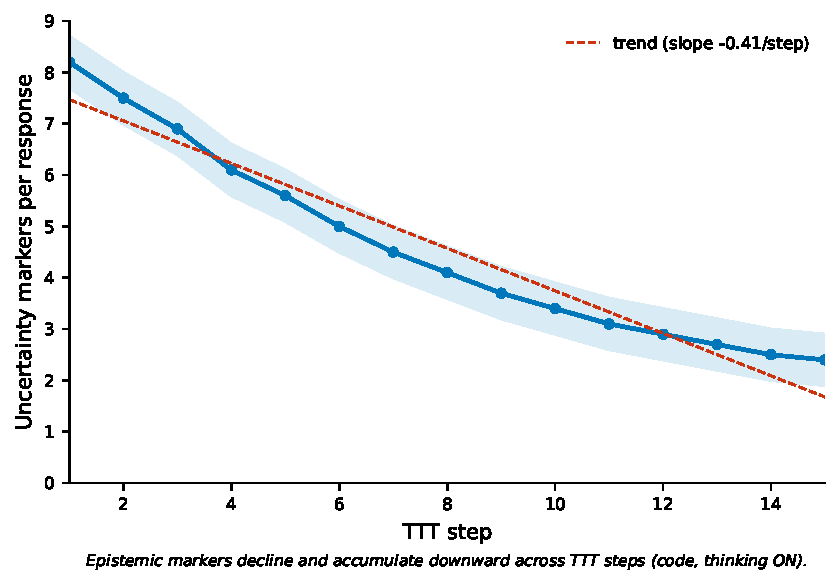
\includegraphics[width=0.82\linewidth]{../figures/bc_fig4_epistemic.pdf}
\caption{Sự đè nén epistemic (RO2). Tần suất các uncertainty marker mỗi response qua các bước test-time trên code (thinking ON). Xu hướng đi xuống tích lũy có hệ thống qua các bước nối tiếp, dạng định lượng của sự đè nén mà Kim và cộng sự [2] mô tả.}
\label{fig:bc-epistemic}
\end{figure}

\section{Ranh giới miền (RO3): Đặc trưng hóa kiến trúc trên toán}\label{the-domain-boundary-architectural-characterization-on-math}

Khác hẳn với sự cất cánh thành công quan sát được ở miền code, đánh giá toán học trên bộ dữ liệu AIME 2026 lại phơi bày một ranh giới hiệu năng khá cứng: mô hình không thoát nổi khỏi trạng thái zero-reward. Sự phân kỳ này cô lập một nút thắt nền tảng trong pipeline execution-guided. Khác với sinh mã — nơi output mục tiêu là một thủ tục thuật toán, được kiểm chứng qua các output test nhiều case dày — bộ AIME chỉ cho một giá trị số tĩnh duy nhất làm feedback, không hề có suy dẫn từng bước hay lời giải kèm theo.

Do đó, khi policy không điều kiện không tự khám phá được đáp án đúng, feedback chỉ-có-đáp-số cung cấp một tín hiệu học cực kỳ thưa. Teacher policy bị ép vào một copy-regime, không trích ra được điều chỉnh thủ tục động nào để distill ngược lại vào student. Trong giới hạn của pilot nhỏ này, điều đó cho thấy hiệu lực của teacher-first self-distillation phụ thuộc nghiêm ngặt vào việc privileged context có truyền tải một thủ tục tái lập được hay chỉ là một giá trị thô — và để lại một khoảng cải thiện then chốt cho feedback toán mang tính thủ tục.

\begin{longtable}[]{@{}
  >{\raggedright\arraybackslash}p{(\columnwidth - 4\tabcolsep) * \real{0.3333}}
  >{\raggedright\arraybackslash}p{(\columnwidth - 4\tabcolsep) * \real{0.3333}}
  >{\raggedright\arraybackslash}p{(\columnwidth - 4\tabcolsep) * \real{0.3333}}@{}}
\caption{Ranh giới value-versus-procedure: kết quả escape-zero theo miền và loại feedback.}\\
\toprule\noalign{}
\begin{minipage}[b]{\linewidth}\raggedright
điều kiện miền
\end{minipage} & \begin{minipage}[b]{\linewidth}\raggedright
nội dung feedback
\end{minipage} & \begin{minipage}[b]{\linewidth}\raggedright
escape-zero?
\end{minipage} \\
\midrule\noalign{}
\endfirsthead
\toprule\noalign{}
\begin{minipage}[b]{\linewidth}\raggedright
điều kiện miền
\end{minipage} & \begin{minipage}[b]{\linewidth}\raggedright
nội dung feedback
\end{minipage} & \begin{minipage}[b]{\linewidth}\raggedright
escape-zero?
\end{minipage} \\
\midrule\noalign{}
\endhead
\bottomrule\noalign{}
\endlastfoot
LiveCodeBench v6 (Code) & Output test nhiều case dày & \textbf{Có (Cải thiện đáng kể)} \\
Pilot AIME 2026 (Toán) & Chỉ một giá trị số tĩnh & Không (Kẹt ở 0/2) \\
\end{longtable}

\section{Pilot toán}\label{math-pilot}

Chạy lại pilot AIME càng làm sắc nét thêm ranh giới thực nghiệm này: trên các bài vượt-năng-lực, teacher chỉ sinh ra toàn bản sao chép, và judge từ chối chúng một cách đúng đắn và triệt để. Vì vậy student không nhận được tín hiệu học nào và kẹt nguyên ở 0. Đây là một minh chứng thực nghiệm khá sạch cho thấy bộ lọc hành xử đúng như thiết kế, đồng thời xác nhận rằng chế độ thất bại trên toán về cơ bản bị ràng buộc bởi sự khan hiếm tín hiệu học của reference và quy mô compute hiện tại, chứ không phải một artifact của pipeline huấn luyện.
